\chapter{Circuit linéaire en régime sinusoïdal forcé (RSF)}
\section{Notation}

\begin{definition}[Sinusoïdal]
    Une sinsoidal est une fonction qui peut s'écrire : 
    \[
        x(t) = X_{m} \cos \left( \omega t + \varphi \right)
    \]
    Avec \(X_{m}\) l'amplitude, \(\omega\) la pulsation et \(\varphi\) la phase à l'origine.   
\end{definition}

\begin{definition}[La valeur moyenne et valeur efficace]
    La valeur moyenne d'une sinusoïdale est donnée par la formule suivante : 
    \[
        \left< x(t) \right> = \frac{1}{T} \int_{0}^{T} x(t) dt = 0
    \]
    Celle-ci étant la même pour toutes les sinusoïdals, on définit alors la valeur efficace : 
    \[
        X_{eff} = \sqrt{\left< x(t)^{2} \right>}
    \]
\end{definition}

\begin{theorem}[Valeur efficace]
    La valeur efficace d'une sinusoïdale \(x(t)\) est : 
    \[
        X_{eff} = \frac{X_{m}}{\sqrt{2}}
    \]
    \begin{explanation}
        On calule \(X_{eff}^{2}\) : 
        \begin{eqnarray*}
            X_{eff}^{2} &=& \left< x(t)^{2} \right> \\
            &=& \frac{1}{T} \int_{0}^{T} x^{2}(t) dt \\
            &=& \frac{1}{T} \int_{0}^{T} X_{m}^{2}\cos^{2}(\omega t + \varphi) dt \\
            &=& \frac{X_{m}^{2}}{T} \int_{0}^{T} \cos^{2}(\omega t + \varphi) dt \\
            \text{ Or :  } \cos^{2}(\theta) &=& \frac{1+\cos(2\theta)}{2} \\
            &=& \frac{X_{m}^{2}}{T} \left( \int_{0}^{T} \frac{1}{2} dt + \int_{0}^{T} \frac{1}{2}\cos(2\omega t + 2\varphi) dt \right) \\
            \text{ Or l'intégrale d'un cosinus } && \text{est nulle sur sa période, d'où : }\\
            X_{eff}^{2} &=& \frac{X_{m}^{2}}{T} \cdot \frac{T}{2} \\
            &=& \frac{X_{m}^{2}}{2} \\
            \implies X_{eff} &=& \frac{X_{m}}{\sqrt{2}} \,\square
        \end{eqnarray*}
    \end{explanation}
\end{theorem}

\begin{lemma}[Grandeur complexe associée à un régime sinusoïdal]
    A une grandeur réelle \(x(t) = X_{m} \cos \omega t + \varphi\), on associe la grandeur complexe \(\underline{x}(t) = X_{m}e^{ j(\omega t + \varphi) }\) avec \(j^{2} = -1\) et \(x(t) = \Re (\underline{x}(t))\). On appelle \(\underline{X}_{m} = X_{m}e^{ j \varphi }\) l'amplitude complexe de \(\underline{x}_{t}\). On a alors : 
    \[
        \underline{x}(t) = \underline{X}_{m}e^{ j \omega t }
    \]    
    Ainsi, 
    \[
        \begin{cases}
            X_{m} = \lvert \underline{X}_{m} \rvert \\
            \varphi = \arg (\underline{X}_{m})
        \end{cases}
    \]
\end{lemma}

\begin{remark}[Equivalence des solutions]
    Si une grandeur \(x(t)\) est solution d'une équation linéaire différentielle, alors la grandeur complexe l'est aussi. \par
    De plus,
    \[
        \begin{cases}
            \frac{d}{dt}\underline{x}_{t} = j \omega \underline{x}(t) \\
            \int \underline{x}(t) dt \,  = \frac{1}{j \omega}\underline{x}(t)
        \end{cases}
    \]
\end{remark}

\section{Indépendance complexe}

\begin{theorem}[Loi d'Ohm généralisée]
    Soit \(u(t) = U_{m} \cos (\omega t + \varphi_{u}) \implies \underline{u}(t) = \underline{U}_{m} e^{ j \omega t }\) et \(i(t) = I_{m} \cos (\omega t + \varphi_{i}) \implies \underline{i}(t) = \underline{I}_{m} e^{ j \omega t }\). \par
    On peut alors écire une version généralisée de la loi d'Ohm pour tous les dipoles linéaires (bobine, resistor, condensateur\dots) : 
    \[
        \underline{u}(t) = \underline{z} \cdot \underline{i}(t) \iff \underline{U}_{m} = \underline{Z} \cdot \underline{I}_{m}
    \]
\end{theorem}

\begin{corollary}[Expression de \(\underline{Z}\) ]
    On peut donc écrire  : \(\underline{Z} = R + jS\) où \(R\) est la résistance du dipôle, \(S\) est la réactance et \(\lvert \underline{Z} \rvert = Z  \) est l'impédance du dipôle.
    \begin{eqnarray*}
        \underline{Z} &=& \frac{\underline{U}_{m}}{\underline{I}_{m}} \\
        &=& \frac{U_{m}}{I_{m}} e^{ j (\varphi_{u} - \varphi_{i}) } \\
        &=& Z e^{ j \varphi } \\
        \implies && \begin{cases}
            \lvert \underline{Z} \rvert = Z  = \frac{U_{m}}{I_{m}} \\
            \arg (\underline{Z}) = \varphi = \varphi_{u} - \varphi_{i}
        \end{cases}
    \end{eqnarray*}
\end{corollary}

\begin{definition}[admittance]
    On définit alors une admittance complexe : 
    \[
        \underline{Y} = \frac{1}{\underline{Z}}
    \]
\end{definition}

\begin{eg}[Exemples]
    Pour un résistor, on a \(\underline{Z} = R\). \par
    Que vaut l'impédence d'une bobine? \par
    Pour une bobine idéale, on a : \(u_{L} = L \frac{di}{dt}\). 
    \begin{eqnarray*}
        \implies \underline{u}_{L}(t)  &=& Lj \omega \underline{i}(t) \\
        &=& \underline{Z}_{L} \underline{i}(t) \\
        \implies \underline{Z}_{L} &=& Lj \omega\\
        \implies && \begin{cases}
            \lvert \underline{Z}_{L} \rvert = L \omega \\
            \varphi = \arg \underline{Z}_{l} = \frac{\pi}{2} = \varphi_{u} - \varphi_{i}
        \end{cases}
    \end{eqnarray*}

    \begin{remark}[Cas d'une bobine réelle]
        Pour une bobine réelle, on a \(u_{l}(t)  = L \dot{i}(t)  + r i(t) \)
        \begin{eqnarray*}
            \implies \underline{u}(t) &=& (L \omega j +r) \underline{i}(t) \\
            \implies \underline{Z}_{l} = L \omega j +r \\
            \implies \lvert \underline{Z}_{L} \rvert = \sqrt{r^{2}+ L^{2} \omega^{2}} 
        \end{eqnarray*}
         Or \(\omega = 2 \pi f \), donc l'impédance augmente avec la fréquence. 
    \end{remark}

    Que vaut l'impédance du condensateur? \par
    Pour le condensateur idéal, 
    \begin{eqnarray*}
        i(t) &=& C\dot{u}(t) \\
        \implies \underline{u}_{l}(t) &=& \frac{1}{jc \omega}\underline{i}(t) \\
        \impliedby \underline{Z}_{C} = \frac{1}{jc \omega} \\
        \implies \begin{cases}
            \lvert \underline{Z}_{c} \rvert = \frac{1}{c \omega} \\
            \varphi = -\frac{\pi}{2} 
        \end{cases}
    \end{eqnarray*}
    
\end{eg}

\begin{theorem}[Equivalence régime continu et RSF]
    L'ensemble des théorèmes du régime continu (loi des noeuds, loi des mailles,\dots) est valable en RSF.
\end{theorem}

\section{Etude d'un circuit RLC en RSF}

\begin{notation}
    Un Générateur de tension alternatif se note : (Voir Schema en dessous)  
\end{notation}

\begin{figure}[!htb]
    \centering
    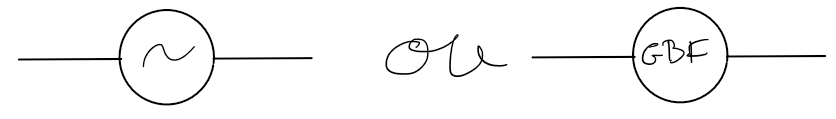
\includegraphics[width=0.5\textwidth]{SCHEMA9.png}
    \caption{Notation d'un générateur de tension alternatif}
    \label{fig:SCHEMA9}
\end{figure}

On construit un circuit RLC avec un générateur de tension alternatif : 
\begin{figure}[!htb]
    \centering
    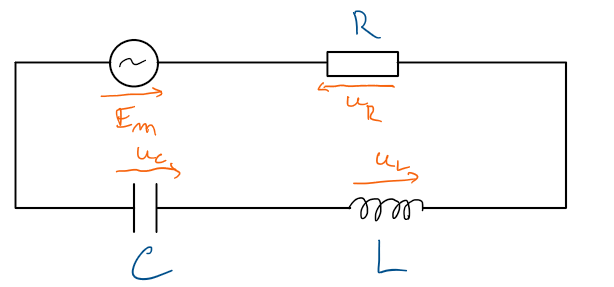
\includegraphics[width=0.5\textwidth]{SCHEMA10.png}
    \caption{Schemadu montage}
    \label{fig:SCHEMA10}
\end{figure}

\begin{theorem}[Loi de Pouillet]
    Dans un circuit en série avec :  un générateur de tension \(E\), un moteur de tension \(E'\) et de résistance \(r\), et deux résistances \(R_{1} \text{ et } R_{2}\), on a : 
    \[
        I = \frac{E-E'}{R_{1}+R_{2}+r}
    \] 
\end{theorem}

\begin{figure}[!htb]
    \centering
    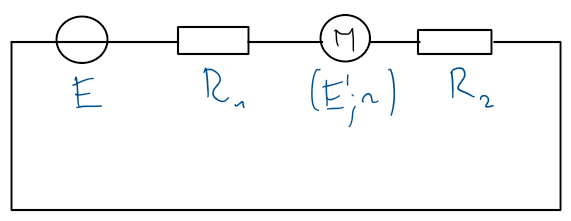
\includegraphics[width=0.5\textwidth]{SCHEMA11.png}
    \caption{Schema de la Loi de Pouillet}
    \label{fig:SCHEMA11}
\end{figure}


Puisque les théorème du régime continu s'appliquent en RSF, on applique la loi de Pouillet : 
\begin{eqnarray*}
    \underline{I}_{m} &=& \frac{\underline{E}_{m}}{\underline{Z}_{R}+ \underline{Z}_{c} + \underline{Z}_{L}} \\
    \implies \underline{E}_{m} &=& \underline{I}_{m} \left( R + j(L \omega - \frac{1}{c \omega}) \right)
\end{eqnarray*}

\subsection{Résonance en intensité aux bords d'un condensateur }

D'après la relation précédente, on a : 
\[
    I_{m} = \lvert \underline{I}_{m} \rvert = \frac{E_{m}}{\sqrt{R^{2} + (L \omega - \frac{1}{c \omega})^{2}}} 
\]

Lorsque \(\omega \to 0\), \(I_{m} \to 0\) et lorsque \(\omega \to  \infty\), \(I_{m} \to 0\). \par
Le numérateur est indépendant de la pulsation \(\omega\), donc l'intensité ne circule que lorsque le dénominateur est minimal, ce qui est le cas pour \(L \omega_{r} - \frac{1}{c \omega_{r}} = 0 \)  
\[
    \implies \omega_{r}^{2} = \frac{1}{LC} = \omega_{\text{0}}^{2}
\]

%SCHEMA

L'équation différentielle du cirquit RLC donne (on note \(u_{c}(t) = u\) ) : 
\begin{eqnarray*}
    L \dot{i} + Ri + u &=& e(t) \\
    LC \ddot{u} + RC \dot{u} + u &=& e(t) \\
    \implies \ddot{u} + \frac{R}{L}\dot{u} + \frac{u}{LC} &=& \frac{e(t)}{LC} \\
    \text{ On pose : } \omega_{\text{0}} = \frac{1}{\sqrt{LC}}\text{ et } \frac{\omega_{\text{0}}}{Q} &=& \frac{R}{L} \\
    \implies Q = \omega_{\text{0}} \frac{L}{R} = \frac{L}{R}\frac{1}{\sqrt{LC}} &=& \frac{1}{R}\sqrt{\frac{L}{C}}
\end{eqnarray*}

\textbf{Il semble me manquer du contenu ici dans la partie sur la résonance en intensité}
